\chapter{Unikernels}
\label{ch:unikernels}

\section{Inleiding}

Dit hoofdstuk zal uitleggen uit welke delen een unikernel bestaat. Tevens wordt er ook beeld gegeven over de voordelen en eigenschappen van unikernels. In het volgende hoofdstuk wordt bekeken welke implementaties van unikernels er al bestaan en wat de verschillen tussen deze implementaties zijn.

Virtuele machines (hoofdstuk \ref{ch:virtualisatie}) zijn er gekomen wanneer men de middelen van computers beter wou gebruiken. Toch werden de middelen niet optimaal benut door de besturingssystemen die werden gebruikt. Bij containers (hoofdstuk \ref{ch:Containers}) wordt het besturingssysteeem van de host machine gedeeld tussen de verschillende software containers. De middelen worden efficiënter gebruikt, doordat er maar één besturingssysteem is.

Unikernels (\cite{madhavapeddy_unikernels_2013}) gaat een andere weg op. Bij unikernels wordt er gekeken naar het besturingssysteem. Traditionele besturingssystemen zoals Ubuntu worden onder de loep genomen. De meeste besturingssystemen die worden gebruikt binnen een productieomgeving, kunnen ook gebruikt worden voor algemene doeleinden.

De eerste implementaties van unikernels worden tegengekomen op het einde van de jaren 90. Exokernel (\cite{mit_mit_1998}) werd ontwikkeld door MIT. De software ontwikkelaars kunnen zelf dus keuzes maken op vlak van abstractie. Nemesis (\cite{university_of_cambridge_nemesis_2000}) werd vanuit de universiteit van Cambridge ontwikkeld. Deze onderzoekers wilden unikernels gebruiken voor doeleinden binnen de multimedia.

Unikernels vragen inzicht in een aantal verschillende technologiëen. De kernel ligt aan de basis van een besturingssysteem en zal in de volgende sectie worden uitgelegd.

\section{Kernel}

De kernel is het programma dat zich centraal bevindt in het besturingssysteem. Het werkt rechtstreeks met de hardware van de computer. De kernel kan gezien worden als het fundament waar het hele besturingssysteem op steunt. Omdat het een belangrijke rol vervult, in het besturingssysteem, is veel van het geheugen van de kernel beveiligd. Dit is bedoeld zodat bepaalde applicaties geen veranderingen kunnen aanbrengen in de kernel. Als er iets fout zou gaan met de kernel, dan heeft dit rechtstreekse gevolgen op het besturingssysteem. Al de handelingen die de kernel uitvoert bevinden zich in de kernel space. Daartegenover gebeurd allles wat de gebruiker uitvoert zich in de user space. Het is van uiterst belang dat de kernel space en user space strikt van elkaar gescheiden zijn. Als dit niet zo zou zijn, dan zou een besturingssysteem niet veilig zijn. De kernel voert nog andere taken uit zoals geheugenbeheer en system calls. Figuur \ref{fig:kernel} toont de positie van de kernel binnen het systeem.

\begin{wrapfigure}{r}{0.3\textwidth}
    \centering
    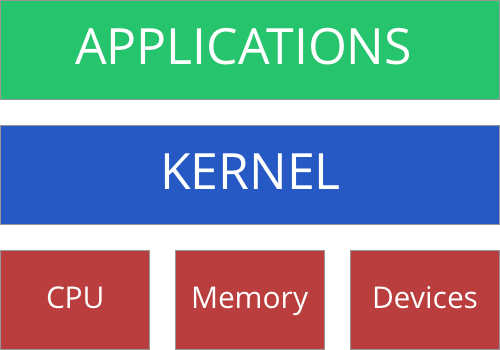
\includegraphics[width=3cm]{img/kernel}
    \caption{positie van kernel tussen de programma's en hardware}
    \label{fig:kernel}
\end{wrapfigure}

Als een programma wordt uitgevoerd, dan bevindt het programma zich binnen de user space. Om het programma in werkelijkheid te kunnen uitvoeren, moet er om toestemming gevraagd worden aan de kernel. Deze instructies moeten worden nagegaan voor de veiligheid. Soms wordt er ook gesproken van memory isolation, waarbij de user space en kernel space niet rechtstreeks met elkaar kunnen communiceren. Dit is een veiligheidsmaatregel.

Volgend boek heeft meer informatie over de werking van de kernel (\cite{bovet_understanding_2005}).

De twee volgende delen zullen de belangrijkste eigenschappen van unikernels uitleggen.

\section{Library besturingssysteem}

Elke virtuele machine binnen de architectuur van een productieomgeving heeft meestal één functie. Dit is al getoond in figuur \ref{fig:virtualmachine}. Elke guest heeft een gespecialiseerde rol om de middelen, dat het ter beschikking krijgt, optimaal te benutten.
Dezelfde architectuur en denkwijze kan teruggevonden worden bij containers. De besturingssystemen, die virtuele machines en containers gebruiken, kan traditioneel worden genoemd. Dit is aangehaald in \cite{madhavapeddy_unikernels_2013}.

Als er dieper wordt ingegaan op deze evolutie, dan kunnen we een patroon vaststellen: er worden steeds kleinere eenheden gebruikt. Eerst was de machine de eenheid en dan de virtuele machine. In het geval van software containers is de eenheid een container. Een unikernel kan ook bekeken worden als een eenheid binnen dit patroon.

Het meest gebruikte besturingssysteem voor servers is het Ubuntu besturingssysteem (\cite{matthias_gelbmann_ubuntu_2016}) met 32\%. Veel applicaties van databases tot en met web applicaties gebruiken het. Dit terwijl een database en een web applicatie andere middelen en functionaliteit nodig hebben.
Er zijn er ook gespecialiseerde besturingssystemen zoals Mini-OS (\cite{satya_popuri_tour_????}). Mini-OS gebruikt veel van de overbodige functies van een traditioneel besturingssysteem niet. Deze gespecialiseerde besturingssystemen zijn in de minderheid en ook niet zeer gekend.

Traditionele besturingssystemen zijn niet de basis die men nodig heeft in een architectuur waar elke eenheid één rol heeft. Alpine (\cite{alpine_linux_development_team_alpine_????}) is een Linux besturingssysteem dat een zeer minimale basis heeft. Tevens beschikt het over een uitgebreide package repository. Dit maakt het een ideaal besturingssysteem voor de basis van software containers. Er kan gestart worden met een kleine basis en alle onderdelen toevoegen die nodig zijn. Dit zorgt voor een container met een kleinere omvang. Hier wordt verder over uitgeweid in sectie \ref{sec:bene_unikernels}.

\begin{wrapfigure}{r}{0.4\textwidth}
    \centering
    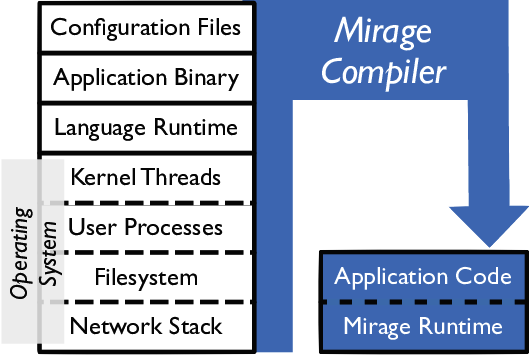
\includegraphics[width=6cm]{img/unikernel}
    \caption{algemeen besturingssysteem tegenover een unikernel implementatie \cite{madhavapeddy_unikernels_2013}}
    \label{fig:unikernel}
\end{wrapfigure}

Sommige onderdelen van het besturingssysteem hebben geen nut meer. Dit kan voor slechtere prestaties en lagere veiligheid zorgen.

Het concept van library besturingssystemen (\cite{madhavapeddy_unikernels_2013}) neemt dit nog een stap verder. Er wordt met een absoluut minimale basis gestart. Daarna worden alleen de componenten toegevoegd, die nodig zijn voor de functionaliteit die de eenheid uitvoert. Library duidt op de verschillende onderdelen of componenten die kunnen worden toegevoegd.

Web applicaties hebben verschillende functies nodig om te kunnen communiceren. Hiervoor bestaan netwerkprotocollen. TCP is een kritiek protocol om te communiceren met het internet en andere apparaten. Bij algemene besturingssystemen, zoals Ubuntu, is dit al aanwezig. Omdat er gestart wordt met een minimale basis, moeten deze protocollen geïmplementeerd worden. Gelukkig zijn er libraries die hiervoor kunnen gebruikt worden. De libraries, broncode en configuratie worden dan gecompileerd. Als resultaat heb je dan een image. Wanneer deze image wordt uitgevoerd dan hebben we een werkende unikernel. De unikernel wordt gecompileerd voor één omgeving en kan alleen gebruikt worden op deze omgeving. Dit is een verschil met software containers en virtuele machines die meer los staan van de omgeving waarin ze zich bevinden.

Unikernels kunnen enkel werken op de omgeving waarvoor ze gecompileerd zijn. Dit is omdat drivers voor de hardware componenten moeten worden geschreven. Kleine veranderingen in de specificatie of interface van een hardware component zorgt ervoor dat de driver niet meer werkt. Drivers zijn één van de grootste obstakels die worden vastgesteld bij library besturingssystemen. Hypervisors lossen dit probleem op door een standaard interface open te stellen. Zo moet er alleen maar één driver worden geschreven voor de hardware component. het werk wordt uitermate verminderd door dit. De protocollen, waar eerder over gesproken is, vormt dan nog een deel van het werk.

\section{Single Address Space}

In een unikernel bestaat er geen concept van user of kernel space. Alle processen bevinden zich binnen dezelfde space. Dit zou problemen geven bij traditionele besturingssystemen. Maar bij het compileren van de unikernel wordt de broncode, libraries en configuratie gecontroleerd. Dit is om te kijken of er zich geen problemen kunnen voordoen. De afwezigheid van de communicatie tussen de kernel en user spaces zorgt voor betere prestaties. Deze verbetering van de prestatie komt ook doordat de hardware kan worden aangesproken zonder dat er veranderd moet worden van context.

Eén globale address space zorgt voor problemen met de isolatie van processen. Meerdere programma's naast elkaar laten werken op een library besturingssysteem is complex. De hypervisor lost dit probleem gedeeltelijk op. Een mogelijke oplossing voor dit probleem wordt verder besproken in Hoofdstuk \ref{ch:microservices}.

\section{Veiligheid}

De hoge mate van veiligheid van unikernels is een gevolg van de specialisatie van de eenheid. Bij virtuele machines en software containers zijn traditionele besturingssystemen de basis. Deze besturingssystemen hebben zeer veel functionaliteit die niet nodig is voor de specifieke taak dat ze uitvoeren. De overbodige functionaliteit kan zorgen voor een lagere prestatie, maar ook voor meer veiligheidsrisico's. Het is dus gemakkelijker om de veiligheid te garanderen van een kleinere broncode tegenover een grote. Daar komt nog bij dat er unikernel implementaties worden gebruikt die specifiek zijn voor de omgeving. Het vraagt veel meer moeite om een gespecialiseerde implementatie te schrijven tegenover een algemene implementatie. Het marktaandeel van de algmene implementatie zal ook veel groter zijn tegenover de specifieke implementatie.

Verder heeft een unikernel geen shell of een andere mogelijkheid om een unikernel aan te passen terwijl deze aan het werken is. Eén unikernel overnemen heeft geen gevolg op de andere unikernels. Daarbij komt nog dat de hypervisors zelf meer veiligheid garanderen (\cite{colp_breaking_2011}).

\section{Andere voordelen}
\label{sec:bene_unikernels}

De omvang van een unikernel is kleiner dan een virtuele machine of een container. Zoals er al eerder werd aangehaald kunnen containers ook een kleine omvang hebben wanneer ze een miniem besturingssysteem gebruiken. Een voorbeeld daarvan is Alpine dat start vanaf 5 MB (\cite{_gliderlabs/docker-alpine_????}).
Een voorbeeld van de omvang van een unikernel kan gevonden worden in \cite[hoofdstuk 4, p.~10]{madhavapeddy_jitsu:_2015} met 1 MB.

Het systeem optimaliseren kan ook in veel grotere mate gebeuren (\cite{madhavapeddy_turning_2010}) dan bij traditionele besturingssystemen.

\section{Productie}

Veel van de commentaar die gegeven wordt op unikernels komt van de moeilijkheden om te kijken wat er fout gaat in productie (\cite{bryan_cantrill_unikernels_2016}). Aanpassingen doen in productie om problemen te verhelpen is niet de beste manier om iets op te lossen. Het programma moet uitgebreid getest worden vooraleer het in de productieomgeving wordt opgesteld. Wanneer er dan toch iets fout gaat in productie, dan zal men de situatie proberen na te bootsen in een soortgelijke omgeving. Het terugzetten van een oudere versie van het programma kan helpen om de gebruikers geen ongemak te laten ondervinden.

\section{Hedendaags gebruik}

Unikernels kunnen momenteel gebruikt worden in beperkte situaties. Er was hetzelfde fenomeen te vinden bij software containers een paar jaar geleden, vooraleer Docker op de voorgrond trad. Elke technologie moet een bepaalde tijd ondergaan om matuur te worden.

In het volgende deel zullen we implementaties van verschillende unikernels vergelijken om een beter beeld te krijgen van de huidige mogelijkheden en het huidige landschap.
